%===================================================================================
\chapter{Mathematical Considerations}\label{s:math}
%===================================================================================

% What does CVODES do?
%--------------------
{\cvodes} solves ODE initial value problems (IVPs) in real $N$-space, which we
write in the abstract form
\begin{equation}\label{e:ivp}
  \dot{y} = f(t,y) \, ,\quad y(t_0) = y_0 \, ,
\end{equation}
where $y \in \mbox{\bf R}^N$.
Here we use $\dot{y}$ to denote $dy/dt$.  While we use $t$ to denote
the independent variable, and usually this is time, it certainly need
not be.  {\cvodes} solves both stiff and nonstiff systems.  Roughly
speaking, stiffness is characterized by the presence of at least one
rapidly damped mode, whose time constant is small compared to the time
scale of the solution itself.

Additionally, if (\ref{e:ivp}) depends on some parameters $p \in {\bf R}^{N_p}$,
i.e.
\begin{equation}\label{e:ivp_p}
\begin{split}
&{\dot{y}}  = f(t,\,y,\,p) \\
&y(t_0)  = y_0(p) \, ,
\end{split}
\end{equation}
{\cvodes} can also compute first order derivative information, performing either
{\em forward sensitivity analysis} or {\em adjoint sensitivity analysis}.
In the first case, {\cvodes} computes the sensitivities of the
solution with respect to the parameters $p$, while in the second case,
{\cvodes} computes the gradient of a {\em derived function} with
respect to the parameters $p$.

%------------------------
\section{IVP solution}\label{ss:ivp_sol}
%------------------------

% Linear multistep methods
%-------------------------
The methods used in {\cvodes} are variable-order, variable-step multistep
methods, based on formulas of the form
\begin{equation}\label{e:lmm}
 \sum_{i = 0}^{K_1} \alpha_{n,i} y^{n-i} +
     h_n \sum_{i = 0}^{K_2} \beta_{n,i} {\dot{y}}^{n-i} = 0 \, .
\end{equation}
Here the $y^n$ are computed approximations to $y(t_n)$, and
$h_n = t_n - t_{n-1}$ is the step size.  The user of {\cvode} must choose
appropriately one of two multistep methods.  For nonstiff problems,
{\cvode} includes the Adams-Moulton formulas\index{Adams method},
characterized by $K_1 = 1$
and $K_2 = q-1$ above, where the order $q$ varies between $1$ and $12$.
For stiff problems, {\cvodes} includes the Backward Differentiation
Formulas (BDF)  \index{BDF method}
in so-called fixed-leading coefficient (FLC) form, given by
$K_1 = q$ and $K_2 = 0$, with order $q$ varying between $1$ and $5$.
The coefficients are uniquely determined by the method type, its
order, the recent history of the step sizes, and the normalization
$\alpha_{n,0} = -1$.  See \cite{ByHi:75} and \cite{JaSD:80}.

% Nonlinear system
%-----------------
\index{nonlinear system!definition|(}
For either choice of formula, a nonlinear system must be solved (approximately)
at each integration step. This nonlinear system can be formulated as
either a rootfinding problem
\begin{equation}\label{e:nonlinear}
  F(y^n) \equiv y^n - h_n \beta_{n,0} f(t_n,y^n) - a_n = 0 \, ,
\end{equation}
or as a fixed-point problem
\begin{equation}\label{e:nonlinear_fixedpoint}
  G(y^n) \equiv h_n \beta_{n,0} f(t_n,y^n) + a_n = y^n \, .
\end{equation}
where $a_n\equiv\sum_{i>0}(\alpha_{n,i}y^{n-i}+h_n\beta_{n,i} {\dot{y}}^{n-i})$.
{\cvodes} provides several nonlinear solver choices as well as the option of
using a user-defined nonlinear solver (see Chapter \ref{c:sunnonlinsol}). By
default {\cvodes} solves (\ref{e:nonlinear}) with a \textit{Newton iteration}
which requires the solution of linear systems
\begin{equation}\label{e:Newton}
  M [y^{n(m+1)} - y^{n(m)}] = -F(y^{n(m)}) \, ,
\end{equation}
in which
\begin{equation}\label{e:Newtonmat}
  M \approx I - \gamma J \, ,
  \quad J = \partial f / \partial y \, ,
  \quad \mbox{and} \quad
  \gamma = h_n \beta_{n,0} \, .
\end{equation}
The exact variation of the Newton iteration depends on the choice of linear
solver and is discussed below and in \S\ref{s:sunnonlinsol_newton}. For nonstiff
systems, a \textit{fixed-point iteration} (previously referred
to as a functional iteration in this guide) for solving
(\ref{e:nonlinear_fixedpoint}) is also available. This involves evaluations of
$f$ only and can (optionally) use Anderson's method \cite{Anderson65,
Walker-Ni09, Fang-Saad09, LWWY11} to accelerate convergence (see
\S\ref{s:sunnonlinsol_fixedpoint} for more details). For any nonlinear solver,
the initial guess for the iteration is a predicted value $y^{n(0)}$ computed
explicitly from the available history data.
\index{nonlinear system!definition|)}

For nonlinear solvers that require the solution of the linear system
(\ref{e:Newton}) (e.g., the default Newton iteration), {\cvodes} provides several
linear solver choices, including the option of a user-supplied linear solver
module (see Chapter \ref{s:sunlinsol}). The linear solver modules distributed
with {\sundials} are organized in two families, a {\em direct} family comprising
direct linear solvers for dense, banded, or sparse matrices, and a {\em spils}
family comprising scaled preconditioned iterative (Krylov) linear solvers.
%%
The methods offered through these modules are as follows:
\begin{itemize}
\item dense direct solvers, using either an internal implementation or
  a BLAS/LAPACK implementation (serial or threaded vector modules only),
\item band direct solvers, using either an internal implementation or
  a BLAS/LAPACK implementation (serial or threaded vector modules only),
\item sparse direct solver interfaces, using either the KLU sparse solver
  library \cite{DaPa:10,KLU_site}, or the thread-enabled SuperLU\_MT sparse
  solver library \cite{Li:05,DGL:99,SuperLUMT_site} (serial or threaded
  vector modules only) [Note that users will need to download and install the
  {\klu} or {\superlumt} packages independent of {\cvodes}],
\item {\spgmr}, a scaled preconditioned GMRES (Generalized Minimal Residual method)
  solver,
\item {\spfgmr}, a scaled preconditioned FGMRES (Flexible Generalized
  Minimal Residual method) solver,
\item {\spbcg}, a scaled preconditioned Bi-CGStab (Bi-Conjugate Gradient Stable
  method) solver,
\item {\sptfqmr}, a scaled preconditioned TFQMR (Transpose-Free Quasi-Minimal
  Residual method) solver, or
\item {\pcg}, a scaled preconditioned CG (Conjugate Gradient method) solver.
\end{itemize}
For large stiff systems, where direct methods are often not feasible, the
combination of a BDF integrator and a preconditioned Krylov
method yields a powerful tool
because it combines established methods for stiff integration,
nonlinear iteration, and Krylov (linear) iteration with a
problem-specific treatment of the dominant source of stiffness, in the
form of the user-supplied preconditioner matrix \cite{BrHi:89}.

In addition, {\cvode} also provides a linear solver module which only uses
a diagonal approximation of the Jacobian matrix.

Note that the dense, band, and sparse direct linear solvers can only be
used with the serial and threaded vector representations.  The
diagonal solver can be used with any vector representation.

% WRMS Norm
%----------
\index{weighted root-mean-square norm|(}
In the process of controlling errors at various levels, {\cvodes} uses a
weighted root-mean-square norm, denoted $\|\cdot\|_{\mbox{\scriptsize WRMS}}$,
for all error-like quantities.  The multiplicative weights used are
based on the current solution and on the relative and absolute
tolerances input by the user, namely
\index{tolerances}
\begin{equation}\label{e:errwt}
 W_i = 1 / [\mbox{\sc rtol} \cdot |y_i| + \mbox{\sc atol}_i ] \, .
\end{equation}
Because $1/W_i$ represents a tolerance in the component $y_i$, a vector
whose norm is 1 is regarded as ``small.''  For brevity, we will
usually drop the subscript WRMS on norms in what follows.
\index{weighted root-mean-square norm|)}

% Newton iteration
%-----------------
\index{nonlinear system!Newton iteration|(}
In the cases of a matrix-based linear solver, the
default Newton iteration is a Modified Newton iteration, in that the iteration matrix
$M$ is fixed throughout the nonlinear iterations.  However, in the
case that a matrix-free iterative linear solver is used, the default
Newton iteration is an Inexact Newton iteration, in which $M$ is
applied in a matrix-free manner, with matrix-vector products $Jv$
obtained by either difference quotients or a user-supplied routine.
With the default Newton iteration, the matrix $M$ and preconditioner
matrix $P$ are updated as infrequently as possible to balance the high
costs of matrix operations against other costs.  Specifically, this matrix
update occurs when:
\begin{itemize}
\item starting the problem,
\item more than 20 steps have been taken since the last update,
\item the value $\bar{\gamma}$ of $\gamma$ at the last update
satisfies $|\gamma/\bar{\gamma} - 1| > 0.3$,
\item a non-fatal convergence failure just occurred, or
\item an error test failure just occurred.
\end{itemize}
When forced by a convergence failure, an update of $M$ or $P$ may or
may not involve a reevaluation of $J$ (in $M$) or of Jacobian data
(in $P$), depending on whether Jacobian error was the likely cause of
the failure.  More generally, the decision is made to reevaluate $J$
(or instruct the user to reevaluate Jacobian data in $P$) when:
\begin{itemize}
\item starting the problem,
\item more than 50 steps have been taken since the last evaluation,
\item a convergence failure occurred with an outdated matrix, and
the value $\bar{\gamma}$ of $\gamma$ at the last update
satisfies $|\gamma/\bar{\gamma} - 1| < 0.2$, or
\item a convergence failure occurred that forced a step size reduction.
\end{itemize}
\index{nonlinear system!Newton iteration|)}

% Convergence test
%------------------------
\index{nonlinear system!Convergence test|(}
The default stopping test for nonlinear solver iterations is related to the
subsequent local error test, with the goal of keeping the nonlinear
iteration errors from interfering with local error control.  As
described below, the final computed value $y^{n(m)}$ will have to
satisfy a local error test $\|y^{n(m)} - y^{n(0)}\| \leq \epsilon$.
Letting $y^n$ denote the exact solution of (\ref{e:nonlinear}), we want
to ensure that the iteration error $y^n - y^{n(m)}$ is small relative
to $\epsilon$, specifically that it is less than $0.1 \epsilon$.
(The safety factor $0.1$ can be changed by the user.)  For this, we
also estimate the linear convergence rate constant $R$ as follows.
We initialize $R$ to 1, and reset $R = 1$ when $M$ or $P$ is updated.
After computing a correction $\delta_m = y^{n(m)}-y^{n(m-1)}$, we
update $R$ if $m > 1$ as
\begin{equation*}
  R \leftarrow \max\{0.3R , \|\delta_m\| / \|\delta_{m-1}\| \} \, .
\end{equation*}
Now we use the estimate
\begin{equation*}
  \| y^n - y^{n(m)} \| \approx \| y^{n(m+1)} - y^{n(m)} \|
  \approx R \| y^{n(m)} - y^{n(m-1)} \|  =  R \|\delta_m \| \, .
\end{equation*}
Therefore the convergence (stopping) test is
\begin{equation*}
  R \|\delta_m \| < 0.1 \epsilon \, .
\end{equation*}
We allow at most 3 iterations (but this limit can be changed by the
user).  We also declare the iteration diverged if any $\|\delta_m\| /
\|\delta_{m-1}\| > 2$ with $m > 1$. If convergence fails with $J$ or
$P$ current, we are forced to reduce the step size, and we replace
$h_n$ by $h_n/4$.  The integration is halted after a preset number
of convergence failures; the default value of this limit is 10,
but this can be changed by the user.
\index{nonlinear system!Convergence test|)}

When an iterative method is used to solve the linear system, its
errors must also be controlled, and this also involves the local error
test constant.  The linear iteration error in the solution vector
$\delta_m$ is approximated by the preconditioned residual vector.
Thus to ensure (or attempt to ensure) that the linear iteration errors
do not interfere with the nonlinear error and local integration error
controls, we require that the norm of the preconditioned residual
be less than $0.05 \cdot (0.1 \epsilon)$.

% Jacobian DQ approximations
%---------------------------
When the Jacobian is stored using either dense or band {\sunmatrix}
objects, the Jacobian may be supplied by a user routine, or
approximated by difference quotients, at the user's option.  In the
latter case, we use the usual approximation
\[ J_{ij} = [f_i(t,y+\sigma_j e_j) - f_i(t,y)]/\sigma_j \, . \]
The increments $\sigma_j$ are given by
\[ \sigma_j = \max\left\{\sqrt{U} \; |y_j| , \sigma_0 / W_j \right\} \, , \]
where $U$ is the unit roundoff, $\sigma_0$ is a dimensionless value,
and $W_j$ is the error weight defined in (\ref{e:errwt}).  In the dense
case, this scheme requires $N$ evaluations of $f$, one for each column
of $J$.  In the band case, the columns of $J$ are computed in groups,
by the Curtis-Powell-Reid algorithm, with the number of $f$ evaluations
equal to the bandwidth.

We note that with sparse and user-supplied {\sunmatrix} objects, the
Jacobian {\em must} be supplied by a user routine.

In the case of a Krylov method, preconditioning may be used on the left, on the
right, or both, with user-supplied routines for the preconditioning
setup and solve operations, and optionally also for the required
matrix-vector products $Jv$.  If a routine for $Jv$ is not supplied,
these products are computed as
\begin{equation}\label{jacobv}
Jv = [f(t,y+\sigma v) - f(t,y)]/\sigma \, .
\end{equation}
The increment $\sigma$ is $1/\|v\|$, so that $\sigma v$ has norm 1.

% Error test
%-----------
\index{error control!step size selection|(}
A critical part of {\cvodes} --- making it an ODE ``solver'' rather than
just an ODE method, is its control of local error.  At every step, the
local error is estimated and required to satisfy tolerance conditions,
and the step is redone with reduced step size whenever that error test
fails.  As with any linear multistep method, the local truncation
error LTE, at order $q$ and step size $h$, satisfies an asymptotic
relation
\[ \mbox{LTE} = C h^{q+1} y^{(q+1)} + O(h^{q+2}) \]
for some constant $C$, under mild assumptions on the step sizes.
A similar relation holds for the error in the predictor $y^{n(0)}$.
These are combined to get a relation
\[ \mbox{LTE} = C' [y^n - y^{n(0)}] + O(h^{q+2}) \, . \]
The local error test is simply $\|\mbox{LTE}\| \leq 1$.  Using the above,
it is performed on the predictor-corrector difference
$\Delta_n \equiv y^{n(m)} - y^{n(0)}$ (with $y^{n(m)}$ the final
iterate computed), and takes the form
\[ \|\Delta_n\| \leq \epsilon \equiv 1/|C'| \, . \]
If this test passes, the step is considered successful.  If it fails,
the step is rejected and a new step size $h'$ is computed based on the
asymptotic behavior of the local error, namely by the equation
\[ (h'/h)^{q+1} \|\Delta_n\| = \epsilon/6 \, . \]
Here 1/6 is a safety factor.  A new attempt at the step is made,
and the error test repeated.  If it fails three times, the order $q$
is reset to 1 (if $q > 1$), or the step is restarted from scratch (if
$q = 1$).  The ratio $h'/h$ is limited above to 0.2 after two error test
failures, and limited below to 0.1 after three.  After seven failures,
{\cvodes} returns to the user with a give-up message.
\index{error control!step size selection|)}

% Step/order control
%-------------------
\index{error control!order selection|(}
In addition to adjusting the step size to meet the local error test,
{\cvode} periodically adjusts the order, with the goal of maximizing the
step size.  The integration starts out at order 1 and varies the order
dynamically after that.  The basic idea is to pick the order $q$ for
which a polynomial of order $q$ best fits the discrete data involved
in the multistep method.  However, if either a convergence failure or
an error test failure occurred on the step just completed, no change
in step size or order is done.  At the current order $q$, selecting a
new step size is done exactly as when the error test fails, giving a
tentative step size ratio
\[ h'/h = (\epsilon / 6 \|\Delta_n\| )^{1/(q+1)} \equiv \eta_q \, . \]
We consider changing order only after taking $q+1$ steps at order $q$,
and then we consider only orders $q' = q - 1$ (if $q > 1$) or
$q' = q + 1$ (if $q < 5$).  The local truncation error at order $q'$
is estimated using the history data.  Then a tentative step size ratio
is computed on the basis that this error, LTE$(q')$, behaves
asymptotically as $h^{q'+1}$.  With safety factors of 1/6 and
1/10 respectively, these ratios are:
\[ h'/h = [1 / 6 \|\mbox{LTE}(q-1)\| ]^{1/q} \equiv \eta_{q-1} \]
and
\[ h'/h = [1 / 10 \|\mbox{LTE}(q+1)\| ]^{1/(q+2)} \equiv \eta_{q+1} \, . \]
The new order and step size are then set according to
\[ \eta = \max\{\eta_{q-1},\eta_q,\eta_{q+1}\} ~,~~ h' = \eta h \, , \]
with $q'$ set to the index achieving the above maximum.
However, if we find that $\eta < 1.5$, we do not bother with the
change.  Also, $h'/h$ is always limited to 10, except on the first
step, when it is limited to $10^4$.
\index{error control!order selection|)}

The various algorithmic features of {\cvodes} described above, as
inherited from {\vode} and {\vodpk}, are documented in
\cite{BBH:89,Byr:92,Hin:00}.  They are also summarized in
\cite{HBGLSSW:05}.

% Additional constraints on y components
%---------------------------------------
{\cvodes} permits the user to impose optional inequality constraints on individual
components of the solution vector $y$. Any of the following four constraints
can be imposed: $y_i > 0$, $y_i < 0$, $y_i \geq 0$, or $y_i \leq 0$.
The constraint satisfaction is tested after a successful nonlinear system solution.
If any constraint fails, we declare a convergence failure of the Newton iteration
and reduce the step size. Rather than cutting the step size by some arbitrary factor,
{\cvodes} estimates a new step size $h'$ using a linear approximation ofthe components
in $y$ that failed the constraint test (including a afety factor of $0.9$ to
cover the strict inequality case).

% Output modes
%-------------
\index{output mode}
Normally, {\cvodes} takes steps until a user-defined output value
$t = t_{\mbox{\scriptsize out}}$ is overtaken, and then it computes
$y(t_{\mbox{\scriptsize out}})$ by interpolation.  However, a
``one step'' mode option is available, where control returns to the
calling program after each step.  There are also options to force
{\cvodes} not to integrate past a given stopping point
$t = t_{\mbox{\scriptsize stop}}$.

%------------------------
\section{Preconditioning}\label{s:preconditioning}
%------------------------
\index{preconditioning!advice on|(}
When using a nonlinear solver that requires the solution of the linear system
(\ref{e:Newton}) (e.g., the default Newton iteration),
{\cvodes} makes repeated use of a linear solver to solve linear systems of the form
$M x = - r$, where $x$ is a correction vector and $r$ is a residual vector.
If this linear system solve is done with one of the scaled preconditioned iterative
linear solvers supplied with {\sundials}, these solvers are rarely successful if used without preconditioning;
it is generally necessary to precondition the system in order to obtain acceptable efficiency.
A system $A x = b$ can be preconditioned on the left, as $(P^{-1}A) x = P^{-1} b$;
on the right, as $(A P^{-1}) P x = b$; or on both sides, as
$(P_L^{-1} A P_R^{-1}) P_R x = P_L^{-1}b$.  The Krylov method is then
applied to a system with the matrix $P^{-1}A$, or $AP^{-1}$, or
$P_L^{-1} A P_R^{-1}$, instead of $A$.  In order to improve the
convergence of the Krylov iteration, the preconditioner matrix $P$, or
the product $P_L P_R$ in the last case, should in some sense
approximate the system matrix $A$.  Yet at the same time, in order to
be cost-effective, the matrix $P$, or matrices $P_L$ and $P_R$, should
be reasonably efficient to evaluate and solve.  Finding a good point
in this tradeoff between rapid convergence and low cost can be very
difficult.  Good choices are often problem-dependent (for example, see
\cite{BrHi:89} for an extensive study of preconditioners for
reaction-transport systems).

Most of the iterative linear solvers supplied with {\sundials} allow
for preconditioning either side, or on both sides, although we know of
no situation where preconditioning on both sides is clearly superior to
preconditioning on one side only (with the product $P_L P_R$).
Moreover, for a given preconditioner matrix, the merits of left vs.~right
preconditioning are unclear in general, and the user should experiment
with both choices.  Performance will differ because the inverse of the
left preconditioner is included in the linear system residual whose
norm is being tested in the Krylov algorithm.  As a rule, however, if
the preconditioner is the product of two matrices, we recommend that
preconditioning be done either on the left only or the right only,
rather than using one factor on each side.

Typical preconditioners used with {\cvodes} are based on approximations
to the system Jacobian, $J = \partial f / \partial y$.  Since the
matrix involved is $M = I - \gamma J$, any
approximation $\bar{J}$ to $J$ yields a matrix that is of potential
use as a preconditioner, namely $P = I - \gamma \bar{J}$.  Because the
linear solver iteration occurs within a nonlinear solver iteration and further also
within a time integration, and since each of these iterations has its
own test for convergence, the preconditioner may use a very crude
approximation, as long as it captures the dominant numerical
feature(s) of the system.  We have found that the combination of a
preconditioner with the Newton-Krylov iteration, using even a fairly
poor approximation to the Jacobian, can be surprisingly superior to
using the same matrix without Krylov acceleration (i.e., a modified
Newton iteration), as well as to using the Newton-Krylov method with
no preconditioning.
\index{preconditioning!advice on|)}


%------------------------
\section{BDF stability limit detection}\label{s:bdf_stab}
%------------------------

\index{Stability limit detection}
{\cvodes} includes an algorithm, {\stald} (STAbility Limit Detection),
which provides protection against potentially unstable behavior of the
BDF multistep integration methods in certain situations, as described below.

When the BDF option is selected, {\cvodes} uses Backward Differentiation
Formula methods of orders 1 to 5.  At order 1 or 2, the BDF
method is A-stable, meaning that for any complex constant $\lambda$ in
the open left half-plane, the method is unconditionally stable (for
any step size) for the standard scalar model problem $\dot{y} = \lambda y$.
For an ODE system, this means that, roughly speaking, as long as all
modes in the system are stable, the method is also stable for any
choice of step size, at least in the sense of a local linear stability
analysis.

At orders 3 to 5, the BDF methods are not A-stable, although they are
{\em stiffly stable}. In each case, in order for the method to be stable
at step size $h$ on the scalar model problem, the product $h\lambda$ must
lie within a {\em region of absolute stability}.
That region excludes a portion of the left half-plane that is concentrated
near the imaginary axis.  The size of that region of instability grows as the order
increases from 3 to 5.  What this means is that, when running BDF at
any of these orders, if an eigenvalue $\lambda$ of the system lies close
enough to the imaginary axis, the step sizes $h$ for which the method is
stable are limited (at least according to the linear stability theory)
to a set that prevents $h\lambda$ from leaving the stability region.
The meaning of {\em close enough} depends on the order.
At order 3, the unstable region is much narrower than at order 5,
so the potential for unstable behavior grows with order.

System eigenvalues that are likely to run into this instability are
ones that correspond to weakly damped oscillations.  A pure undamped
oscillation corresponds to an eigenvalue on the imaginary axis.
Problems with modes of that kind call for different considerations,
since the oscillation generally must be followed by the solver, and
this requires step sizes ($h \sim 1/\nu$, where $\nu$ is the frequency)
that are stable for BDF anyway.  But for a weakly damped oscillatory mode,
the oscillation in the solution is eventually damped to the noise level,
and at that time it is important that the solver not be restricted to step
sizes on the order of $1/\nu$.  It is in this situation that the new option may
be of great value.

In terms of partial differential equations, the typical problems for
which the stability limit detection option is appropriate are
ODE systems resulting from semi-discretized PDEs (i.e., PDEs discretized
in space) with advection and diffusion, but with advection dominating
over diffusion.
Diffusion alone produces pure decay modes, while advection tends to
produce undamped oscillatory modes.  A mix of the two with advection
dominant will have weakly damped oscillatory modes.

The {\stald} algorithm attempts to detect, in a direct
manner, the presence of a stability region boundary that is limiting
the step sizes in the presence of a weakly damped oscillation \cite{Hin:92}.
The algorithm supplements (but differs greatly from) the existing
algorithms in {\cvodes} for choosing step size and order based on
estimated local truncation errors.  The {\stald} algorithm works directly
with history data that is readily available in {\cvodes}.  If it concludes
that the step size is in fact stability-limited, it dictates a
reduction in the method order, regardless of the outcome of the
error-based algorithm.  The {\stald} algorithm has been tested in
combination with the {\vode} solver on linear advection-dominated
advection-diffusion problems \cite{Hin:95}, where it works well.  The
implementation in {\cvodes} has been successfully tested on linear
and nonlinear advection-diffusion problems, among others.

This stability limit detection option adds some computational overhead
to the {\cvodes} solution.  (In timing tests, these overhead costs
have ranged from 2\% to 7\% of the total, depending on the size and
complexity of the problem, with lower relative costs for larger
problems.)  Therefore, it should be activated only when there is
reasonable expectation of modes in the user's system for which it is
appropriate.  In particular, if a {\cvode} solution with this option
turned off appears to take an inordinately large number of steps at
orders 3-5 for no apparent reason in terms of the solution time scale,
then there is a good chance that step sizes are being limited by
stability, and that turning on the option will improve the efficiency
of the solution.


%------------------------
\section{Rootfinding}\label{ss:rootfinding}
%------------------------

\index{Rootfinding}
The {\cvodes} solver has been augmented to include a rootfinding
feature.  This means that, while integrating the Initial Value Problem
(\ref{e:ivp}), {\cvodes} can also find the roots of a set of user-defined
functions $g_i(t,y)$ that depend both on $t$ and on the solution vector
$y = y(t)$.  The number of these root functions is arbitrary, and if
more than one $g_i$ is found to have a root in any given interval, the
various root locations are found and reported in the order that they
occur on the $t$ axis, in the direction of integration.

Generally, this rootfinding feature finds only roots of odd
multiplicity, corresponding to changes in sign of $g_i(t,y(t))$,
denoted $g_i(t)$ for short.  If a user root function has a root of
even multiplicity (no sign change), it will probably be missed by
{\cvodes}.  If such a root is desired, the user should reformulate the
root function so that it changes sign at the desired root.

The basic scheme used is to check for sign changes of any $g_i(t)$ over
each time step taken, and then (when a sign change is found) to hone
in on the root(s) with a modified secant method \cite{HeSh:80}.
In addition, each time $g$ is computed, {\cvodes} checks to see if
$g_i(t) = 0$ exactly, and if so it reports this as a root.  However,
if an exact zero of any $g_i$ is found at a point $t$, {\cvodes}
computes $g$ at $t + \delta$ for a small increment $\delta$, slightly
further in the direction of integration, and if any $g_i(t + \delta)=0$
also, {\cvodes} stops and reports an error.  This way, each time
{\cvodes} takes a time step, it is guaranteed that the values of all
$g_i$ are nonzero at some past value of $t$, beyond which a search for
roots is to be done.

At any given time in the course of the time-stepping, after suitable
checking and adjusting has been done, {\cvodes} has an interval
$(t_{lo},t_{hi}]$ in which roots of the $g_i(t)$ are to be sought, such
that $t_{hi}$ is further ahead in the direction of integration, and
all $g_i(t_{lo}) \neq 0$.  The endpoint $t_{hi}$ is either $t_n$,
the end of the time step last taken, or the next requested output time
$t_{\mbox{\scriptsize out}}$ if this comes sooner.  The endpoint
$t_{lo}$ is either $t_{n-1}$, the last output time
$t_{\mbox{\scriptsize out}}$ (if this occurred within the last
step), or the last root location (if a root was just located within
this step), possibly adjusted slightly toward $t_n$ if an exact zero
was found.  The algorithm checks $g_i$ at $t_{hi}$ for zeros and for
sign changes in $(t_{lo},t_{hi})$.  If no sign changes were found, then
either a root is reported (if some $g_i(t_{hi}) = 0$) or we proceed to
the next time interval (starting at $t_{hi}$).  If one or more sign
changes were found, then a loop is entered to locate the root to
within a rather tight tolerance, given by
\[ \tau = 100 * U * (|t_n| + |h|)~~~ (U = \mbox{unit roundoff}) ~. \]
Whenever sign changes are seen in two or more root functions, the one
deemed most likely to have its root occur first is the one with the
largest value of $|g_i(t_{hi})|/|g_i(t_{hi}) - g_i(t_{lo})|$,
corresponding to the closest to $t_{lo}$ of the secant method values.
At each pass through the loop, a new value $t_{mid}$ is set, strictly
within the search interval, and the values of $g_i(t_{mid})$ are
checked.  Then either $t_{lo}$ or $t_{hi}$ is reset to $t_{mid}$
according to which subinterval is found to include the sign change.  If
there is none in $(t_{lo},t_{mid})$ but some $g_i(t_{mid}) = 0$, then
that root is reported.  The loop continues until
$|t_{hi}-t_{lo}| < \tau$, and then the reported root location is
$t_{hi}$.

In the loop to locate the root of $g_i(t)$, the formula for $t_{mid}$
is
\[ t_{mid} = t_{hi} - (t_{hi} - t_{lo})
             g_i(t_{hi}) / [g_i(t_{hi}) - \alpha g_i(t_{lo})] ~, \]
where $\alpha$ is a weight parameter.  On the first two passes through
the loop, $\alpha$ is set to $1$, making $t_{mid}$ the secant method
value.  Thereafter, $\alpha$ is reset according to the side of the
subinterval (low vs. high, i.e., toward $t_{lo}$ vs. toward $t_{hi}$)
in which the sign change was found in the previous two passes.  If the
two sides were opposite, $\alpha$ is set to 1.  If the two sides were
the same, $\alpha$ is halved (if on the low side) or doubled (if on
the high side).  The value of $t_{mid}$ is closer to $t_{lo}$ when
$\alpha < 1$ and closer to $t_{hi}$ when $\alpha > 1$.  If the above
value of $t_{mid}$ is within $\tau/2$ of $t_{lo}$ or $t_{hi}$, it is
adjusted inward, such that its fractional distance from the endpoint
(relative to the interval size) is between .1 and .5 (.5 being the
midpoint), and the actual distance from the endpoint is at least
$\tau/2$.


%----------------------------------------
\section{Pure quadrature integration}\label{s:quad}
%----------------------------------------

\index{quadrature integration}
In many applications, and most notably during the backward integration phase
of an adjoint sensitivity analysis run (see \S\ref{ss:adj_sensi}) it is of
interest to compute integral quantities of the form
\begin{equation}\label{e:QUAD}
  z(t) = \int_{t_0}^t q(\tau, y(\tau), p) \, d\tau \, .
\end{equation}
The most effective approach to compute $z(t)$ is to extend the original problem
with the additional ODEs (obtained by applying Leibnitz's differentiation rule):
\begin{equation}
  \dot z = q(t,y,p) \, , \quad z(t_0) = 0 \, .
\end{equation}
Note that this is equivalent to using a quadrature method based on the underlying
linear multistep polynomial representation for $y(t)$.

This can be done at the ``user level'' by simply exposing to {\cvodes} the extended 
ODE system (\ref{e:ivp_p})+(\ref{e:QUAD}). However, in the context of an implicit 
integration solver, this approach is not desirable since the nonlinear solver 
module will require the Jacobian (or Jacobian-vector product) of this extended ODE.
Moreover, since the additional states $z$ do not enter the right-hand side of
the ODE (\ref{e:QUAD}) and therefore the right-hand side of the extended ODE system,
it is much more efficient to treat the ODE system (\ref{e:QUAD})
separately from the original system (\ref{e:ivp_p}) by ``taking out'' the additional
states $z$ from the nonlinear system (\ref{e:nonlinear}) that must be solved in
the correction step of the LMM. Instead, ``corrected'' values $z^n$ are computed
explicitly as
\begin{equation*}
  z^n = - \frac{1}{\alpha_{n,0}} \left(
    h_n \beta_{n,0} q(t_n, y_n, p) 
    + h_n \sum_{i=1}^{K_2} \beta_{n,i} \dot z^{n-i}
    + \sum_{i=1}^{K_1} \alpha_{n,i} z^{n-i}
    \right) \, ,
\end{equation*}
once the new approximation $y^n$ is available.

The quadrature variables $z$ can be optionally included in the error test, in 
which case corresponding relative and absolute tolerances must be provided.


%----------------------------------------
\section{Forward sensitivity analysis}\label{ss:fwd_sensi}
%----------------------------------------

\index{forward sensitivity analysis!mathematical background|(}
Typically, the governing equations of complex, large-scale models
depend on various parameters,  through the right-hand side vector 
and/or through the vector of initial conditions, as in (\ref{e:ivp_p}).
In addition to numerically solving the ODEs, it may be desirable to
determine the sensitivity of the results with respect to the model
parameters. 
Such sensitivity information can be used to estimate which
parameters are most influential in affecting the behavior of the
simulation or to evaluate optimization gradients (in the setting of dynamic
optimization, parameter estimation, optimal control, etc.).

The {\em solution sensitivity} with respect to the model parameter
$p_i$ is defined as the vector 
$s_i (t) = {\partial y(t)}/{\partial p_i}$
and satisfies the following {\em forward sensitivity equations}
(or {\em sensitivity equations} for short):
\begin{equation}\label{e:sens_eqns}
{{\dot s}_i}  = \frac{\partial f}{\partial y} s_i + \frac{\partial f}{\partial p_i} \, ,
\quad s_i(t_0)  = \frac{\partial y_{0}(p)}{\partial p_i} \, ,
\end{equation}
obtained by applying the chain rule of differentiation to the original
ODEs~(\ref{e:ivp_p}). 

When performing forward sensitivity analysis, {\cvodes} carries out
the time integration of the combined system, (\ref{e:ivp_p}) and
(\ref{e:sens_eqns}), by viewing it as an ODE system of size
$N(N_s+1)$, where $N_s$ is the number of model parameters $p_i$, with
respect to which sensitivities are desired ($N_s \le N_p$).
However, major improvements in efficiency can be made by taking
advantage of the special form of the sensitivity equations as
linearizations of the original ODEs.  In particular, for stiff
systems, for which {\cvodes} employs a Newton iteration, the original
ODE system and all sensitivity systems share the same Jacobian matrix,
and therefore the same iteration matrix $M$ in (\ref{e:Newtonmat}).

The sensitivity equations are solved with the same linear multistep formula that
was selected for the original ODEs and, if Newton iteration was selected, the
same linear solver is used in the correction phase for both state and sensitivity 
variables. In addition, {\cvodes} offers the option of including
({\em full error control}) or excluding
({\em partial error control}) the sensitivity variables from the local 
error test.

\subsection{Forward sensitivity methods}
\index{forward sensitivity analysis!correction strategies|(}
In what follows we briefly describe three methods that have been proposed for the 
solution of the combined ODE and sensitivity system for the vector
${\hat y} = [y, s_1, \ldots , s_{N_s}]$.

\begin{itemize}

\item {\em Staggered Direct}

  In this approach \cite{CaSt:85}, the nonlinear system
  (\ref{e:nonlinear}) is first solved and, once an acceptable
  numerical solution is obtained, the sensitivity variables at the new
  step are found by directly solving (\ref{e:sens_eqns}) after the
  (BDF or Adams) discretization is used to eliminate ${\dot s}_i$.
  Although the system matrix of the above linear system is based on
  exactly the same information as the matrix $M$ in
  (\ref{e:Newtonmat}), it must be updated and factored at every step
  of the integration, in contrast to an evalutaion of $M$ which is
  updated only occasionally.  For problems with many parameters
  (relative to the problem size), the staggered direct method can
  outperform the methods described below~\cite{LPZ:99}.  However, the
  computational cost associated with matrix updates and factorizations
  makes this method unattractive for problems with many more states
  than parameters (such as those arising from semidiscretization of
  PDEs) and is therefore not implemented in {\cvodes}.
  
\item {\em Simultaneous Corrector}

  In this method \cite{MaPe:97}, the discretization is applied simultaneously
  to both the original equations (\ref{e:ivp_p}) and the sensitivity systems
  (\ref{e:sens_eqns}) resulting in the following nonlinear system 
  \begin{equation*}
    {\hat F}({\hat y}_n) \equiv  
    {\hat y}_n - h_n\beta_{n,0} {\hat f}(t_n,\,{\hat y}_n) - {\hat a}_n = 0 \, ,
  \end{equation*}
  where
  ${\hat f} = [ f(t,y,p), \ldots, (\dfdyI)(t,y,p) s_i + (\dfdpiI)(t,y,p), \ldots ]$,
  and ${\hat a}_n$ is comprised of the terms in the discretization that depend on
  the solution at previous integration steps.
  This combined nonlinear system can be solved using a modified Newton method as in
  (\ref{e:Newton}) by solving the corrector equation
  \begin{equation}\label{e:Newton_sim}
    {\hat M}[{\hat y}_{n(m+1)}-{\hat y}_{n(m)}]=-{\hat F}({\hat y}_{n(m)})
  \end{equation}
  at each iteration, where 
  \begin{equation*}
    {\hat M} = 
    \begin{bmatrix}
      M                &        &        &        &   \\
      - \gamma J_1     & M      &        &        &   \\
      - \gamma J_2     & 0      & M      &        &   \\
        \vdots         & \vdots & \ddots & \ddots &   \\
      - \gamma J_{N_s} & 0      & \ldots & 0      & M 
    \end{bmatrix} \, ,
  \end{equation*}
  $M$ is defined as in (\ref{e:Newtonmat}), and 
  $J_i = ({\partial}/{\partial y})\left[ (\dfdyI) s_i + (\dfdpiI) \right]$.
  It can be shown that 2-step quadratic convergence can be retained by using
  only the block-diagonal portion of ${\hat M}$ in the corrector equation
  (\ref{e:Newton_sim}). This results in a decoupling that allows the reuse of 
  $M$ without additional matrix factorizations. However, the products
  $(\dfdyI)s_i$ and the vectors $\dfdpiI$ must still be reevaluated at 
  each step of the iterative process (\ref{e:Newton_sim}) to update the 
  sensitivity portions of the residual ${\hat G}$.
  
\item {\em Staggered corrector}

  In this approach \cite{FTB:97}, as in the staggered direct method,
  the nonlinear system (\ref{e:nonlinear}) is solved first using the Newton
  iteration (\ref{e:Newton}). Then a separate Newton iteration is used to solve the
  sensitivity system (\ref{e:sens_eqns}):
  \begin{multline}\label{e:stgr_iterations}
    M [s_{i}^{n(m+1)} - s_{i}^{n(m)}]= \\
    - \left[ s_{i}^{n(m)} - 
    \gamma \left( \dfdy (t_n , y^n, p) s_{i}^{n(m)} + \dfdpi (t_n , y^n , p) \right)
    -a_{i,n} \right] \, ,
  \end{multline}
  where $a_{i,n}=\sum_{j>0}(\alpha_{n,j}s_{i}^{n-j}+h_n\beta_{n,j}{{\dot s}_i}^{n-j})$.
  In other words, a modified Newton iteration is used to solve a linear system.
  In this approach, the vectors $\dfdpiI$ need be updated only once per
  integration step, after the state correction phase (\ref{e:Newton}) has
  converged. Note also that Jacobian-related data can be reused at all iterations
  (\ref{e:stgr_iterations}) to evaluate the products $(\dfdyI) s_i$.
\end{itemize}  

{\cvodes} implements the simultaneous corrector method and two flavors of the 
staggered corrector method which differ only if the sensitivity variables are
included in the error control test. \index{error control!sensitivity variables} 
In the {\em full error control} case, the first variant of the staggered corrector
method requires the convergence of the iterations (\ref{e:stgr_iterations}) for
all $N_s$ sensitivity systems and then performs the error test on the sensitivity
variables. The second variant of the method will perform the error test for each
sensitivity vector $s_i, (i=1,2,\ldots,N_s$) individually, as they pass the
convergence test. Differences in performance between the two variants may therefore
be noticed whenever one of the sensitivity vectors $s_i$ fails a convergence or
error test. 

An important observation is that the staggered corrector method, combined with 
a Krylov linear solver, effectively results in a staggered direct method. 
Indeed, the Krylov solver requires only the action of the matrix $M$ on a vector
and this can be provided with the current Jacobian information. Therefore, the
modified Newton procedure (\ref{e:stgr_iterations}) will theoretically converge 
after one iteration.
\index{forward sensitivity analysis!correction strategies|)}

\subsection{Selection of the absolute tolerances for sensitivity variables}
\index{forward sensitivity analysis!absolute tolerance selection|(}
If the sensitivities are included in the error
test\index{error control!sensitivity variables}, {\cvodes} provides an
automated estimation of absolute tolerances for the sensitivity variables 
based on the absolute tolerance for the corresponding state variable.
The relative tolerance for sensitivity variables is set to be the same as for 
the state variables. The selection of absolute tolerances for the sensitivity 
variables is based on the observation that the sensitivity vector $s_i$ will have 
units of $[y]/[p_i]$.
With this, the absolute tolerance for the $j$-th component of the sensitivity
vector $s_i$ is set to ${\mbox{\sc atol}_j}/{|{\bar p}_i|}$, where
$\mbox{\sc atol}_j$ are the absolute tolerances for the state variables and $\bar p$
is a vector of scaling factors that are dimensionally consistent with
the model parameters $p$ and give an indication of their order of magnitude.
This choice of relative and absolute tolerances is equivalent 
to requiring that the weighted root-mean-square norm of the sensitivity 
vector $s_i$ with weights based on $s_i$ be the same as the
weighted root-mean-square norm of the vector of scaled sensitivities 
${\bar s}_i = |{\bar p}_i| s_i$ with weights based on the state variables
(the scaled sensitivities ${\bar s}_i$ being dimensionally consistent with the
state variables).
%
However, this choice of tolerances for the $s_i$ may be a poor one, and the user 
of {\cvodes} can provide different values as an option.
\index{forward sensitivity analysis!absolute tolerance selection|)}

\subsection{Evaluation of the sensitivity right-hand side}
\index{forward sensitivity analysis!right-hand side evaluation}
There are several methods for evaluating the right-hand side of the sensitivity 
systems (\ref{e:sens_eqns}): analytic evaluation, automatic differentiation, 
complex-step approximation, and finite differences (or directional derivatives).
{\cvodes} provides all the software hooks for implementing interfaces to
automatic differentiation (AD) or complex-step approximation; future versions
will include a generic interface to AD-generated functions.
At the present time, besides the option for analytical sensitivity right-hand 
sides (user-provided), {\cvodes} can evaluate these quantities using various
finite difference-based approximations to evaluate the terms $(\dfdyI) s_i$ 
and $(\dfdpiI)$, or using directional derivatives to evaluate
$\left[ (\dfdyI) s_i + (\dfdpiI) \right]$.
As is typical for finite differences, the proper choice of perturbations is a 
delicate matter. {\cvodes} takes into account several problem-related features:
the relative ODE error tolerance $\mbox{\sc rtol}$, the machine unit roundoff $U$,
the scale factor ${\bar p}_i$, and the weighted root-mean-square norm of the 
sensitivity vector $s_i$.

Using central finite differences as an example, the two terms 
$({\partial f}/{\partial y}) s_i$ 
and ${\partial f}/{\partial p_i}$ in the right-hand side of (\ref{e:sens_eqns}) 
can be evaluated either separately:
\begin{gather}
  \frac{\partial f}{\partial y} s_i \approx \frac{f(t, y+\sigma_y s_i, p)-
    f(t, y-\sigma_y s_i, p)}{2\,\sigma_y} \, , \label{e:fd2} \\
  \frac{\partial f}{\partial p_i} \approx \frac{f(t,y,p + \sigma_i e_i)-
    f(t,y,p - \sigma_i e_i)}{2\,\sigma_i} \, , \tag{\ref{e:fd2}'} \\
  \sigma_i = |{\bar p}_i| \sqrt{\max( \mbox{\sc rtol} , U)} \, , \quad
  \sigma_y = \frac{1}{\max(1/\sigma_i, \|s_i\|_{\mbox{\scriptsize WRMS}}/|{\bar p}_i|)} \, , \nonumber
\end{gather}
or simultaneously:
\begin{gather}
  \frac{\partial f}{\partial y} s_i + \frac{\partial f}{\partial p_i} \approx
  \frac{f(t, y+\sigma s_i, p + \sigma e_i) -
    f(t, y-\sigma s_i, p - \sigma e_i)}{2\,\sigma} \, , \label{e:dd2} \\
  \sigma = \min(\sigma_i, \sigma_y) \, , \nonumber
\end{gather}
or by adaptively switching between (\ref{e:fd2})+(\ref{e:fd2}') and (\ref{e:dd2}), 
depending on the relative size of the finite difference increments
$\sigma_i$ and $\sigma_y$.  In the adaptive scheme, if
$\rho = \max(\sigma_i/\sigma_y,\sigma_y/\sigma_i)$, we use separate
evaluations if $\rho > \rhomax$ (an input value), and simultaneous
evaluations otherwise.

These procedures for choosing the perturbations ($\sigma_i$, $\sigma_y$, $\sigma$)
and switching between finite difference and directional derivative
formulas have also been implemented for one-sided difference formulas.
Forward finite differences can be applied to $({\partial f}/{\partial y}) s_i$
and ${\partial f}/{\partial p_i}$ separately, or the single directional
derivative formula
\begin{equation*}
\dfdy s_i + \dfdpi \approx
\frac{f(t, y+\sigma s_i, p + \sigma e_i) - f(t, y, p)}{\sigma}
\end{equation*}
can be used.
In {\cvodes}, the default value of $\rhomax=0$ indicates the use of
the second-order centered directional derivative formula (\ref{e:dd2}) exclusively.
Otherwise, the magnitude of $\rhomax$ and its sign (positive or
negative) indicates whether this switching is done with regard to
(centered or forward) finite differences, respectively.
\index{forward sensitivity analysis!right hand side evaluation|)}


\subsection{Quadratures depending on forward sensitivities}
\index{quadrature integration!forward sensitivity analysis}
If pure quadrature variables are also included in the problem definition
(see \S\ref{s:quad}), {\cvodes} does {\em not} carry their sensitivities 
automatically. Instead, we provide a more general feature through which
integrals depending on both the states $y$ of (\ref{e:ivp_p}) and the
state sensitivities $s_i$ of (\ref{e:sens_eqns}) can be evaluated. In other
words, {\cvodes} provides support for computing integrals of the form:
\begin{equation*}
 \bar z(t) = \int_{t_0}^t \bar q(\tau, y(\tau), s_1(\tau), \ldots, s_{N_p}(\tau),p) \, d\tau \, .
\end{equation*}

If the sensitivities of the quadrature variables $z$ of (\ref{e:QUAD}) are
desired, these can then be computed by using:
\begin{equation*}
  \bar q_i = q_y s_i + q_{p_i} \, , \quad i = 1,\ldots,N_p \, ,
\end{equation*}
as integrands for $\bar{z}$, where $q_y$ and $q_p$ are the partial derivatives
of the integrand function $q$ of (\ref{e:QUAD}).

As with the quadrature variables $z$, the new variables $\bar z$ are also excluded
from any nonlinear solver phase and ``corrected'' values $\bar z^n$ are obtained
through explicit formulas. 
\index{forward sensitivity analysis!mathematical background|)}

%----------------------------------------
\section{Adjoint sensitivity analysis}\label{ss:adj_sensi}
%----------------------------------------
\index{adjoint sensitivity analysis!mathematical background|(}
In the {\em forward sensitivity approach} described in the previous
section, obtaining sensitivities with respect to $N_s$ parameters is roughly
equivalent to solving an ODE system of size $(1+N_s) N$. This can become 
prohibitively expensive, especially for large-scale problems, if sensitivities
with respect to many parameters are desired.
In this situation, the {\em adjoint sensitivity method} is a very
attractive alternative, provided that we do not need the solution sensitivities
$s_i$, but rather the gradients with respect to model parameters of a relatively 
few derived functionals of the solution. In other words, if $y(t)$ is the solution
of (\ref{e:ivp_p}), we wish to evaluate the gradient ${dG}/{dp}$ of
\begin{equation}\label{e:G}
G(p) = \int_{t_0}^T g(t, y, p) dt \, ,
\end{equation}
or, alternatively, the gradient ${dg}/{dp}$ of the function $g(t, y, p)$ 
at the final time $T$. 
The function $g$ must be smooth enough that $\partial g / \partial y$ 
and $\partial g / \partial p$ exist and are bounded. 

In what follows, we only sketch the analysis for the 
sensitivity problem for both $G$ and $g$.
For details on the derivation see \cite{CLPS:03}.
Introducing a Lagrange multiplier $\lambda$, we form the augmented
objective function
\begin{equation}
I(p) = G(p) - \int_{t_0}^T \lambda^* 
\left( {\dot y} - f(t,y,p)\right) dt \, ,
\end{equation}
where $*$ denotes the conjugate transpose. The gradient of $G$ with respect
to $p$ is
\begin{equation}
  \frac{dG}{dp} = \frac{dI}{dp} 
=\int_{t_0}^T(g_p + g_y s)dt - \int_{t_0}^T 
\lambda^* \left( {\dot s} - f_y s - f_p \right)dt \, ,
\end{equation}
where subscripts on functions $f$ or $g$ are used to denote partial 
derivatives and $s = [s_1,\ldots,s_{N_s}]$ is the matrix of solution sensitivities.
Applying integration by parts to the term $\lambda^* {\dot s}$, and by requiring
that $\lambda$ satisfy
\begin{equation}\label{e:adj_eqns}
\begin{split}
&{\dot\lambda} = -\left( \dfdy \right)^* \lambda - 
\left( \frac{\partial g}{\partial y} \right)^* \\
&\lambda(T) = 0 \, ,
\end{split}
\end{equation}
the gradient of $G$ with respect to $p$ is nothing but
\begin{equation}\label{e:dGdp}
\frac{dG}{dp} = \lambda^*(t_0) s(t_0) + 
\int_{t_0}^T \left( g_p + \lambda^* f_p \right) dt \, .
\end{equation}
The gradient of $g(T,y,p)$ with respect to $p$ can be then obtained
by using the Leibnitz differentiation rule. Indeed, from (\ref{e:G}),
\begin{equation*}
\frac{dg}{dp}(T) = \frac{d}{dT}\frac{dG}{dp}
\end{equation*}
and therefore, taking into account that $dG/dp$ in (\ref{e:dGdp}) depends on $T$
both through the upper integration limit and through $\lambda$, and that
$\lambda(T) = 0$, 
\begin{equation}\label{e:dgdp}
\frac{dg}{dp}(T) = \mu^*(t_0) s(t_0) + g_p(T) +
\int_{t_0}^T \mu^* f_p dt \, ,
\end{equation}
where $\mu$ is the sensitivity of $\lambda$ with respect to the final integration 
limit $T$.  Thus $\mu$ satisfies the following equation, obtained by taking the
total derivative with respect to $T$ of (\ref{e:adj_eqns}):
\begin{equation}\label{e:adj1_eqns}
\begin{split}
&{\dot\mu} = -\left( \dfdy \right)^* \mu \\ 
&\mu(T) = \left( \frac{\partial g}{\partial y} \right)^*_{t=T} \, .
\end{split}
\end{equation}
The final condition on $\mu(T)$ follows from 
$(\partial\lambda/\partial t) + (\partial\lambda/\partial T) = 0$ at $T$, and
therefore, $\mu(T) = -{\dot\lambda}(T)$. 

The first thing to notice about the adjoint system (\ref{e:adj_eqns}) is that there
is no explicit specification of the parameters $p$; this implies that, once the
solution $\lambda$ is found, the formula (\ref{e:dGdp}) can then be used to find
the gradient of $G$ with respect to any of the parameters $p$. The same holds true
for the system (\ref{e:adj1_eqns}) and the formula (\ref{e:dgdp}) for gradients of
$g(T,y,p)$.  The second important remark is that the adjoint systems
(\ref{e:adj_eqns}) and (\ref{e:adj1_eqns}) are terminal value problems which depend
on the solution $y(t)$ of the original IVP (\ref{e:ivp_p}). Therefore, a procedure
is needed for providing the states $y$ obtained during a forward integration phase
of (\ref{e:ivp_p}) to {\cvodes} during the backward integration phase of
(\ref{e:adj_eqns}) or (\ref{e:adj1_eqns}).  The approach adopted in {\cvodes},
based on {\em checkpointing}, is described below.

\subsection{Checkpointing scheme}\label{ss:checkpointing}
\index{adjoint sensitivity analysis!checkpointing}
During the backward integration, the evaluation of the right-hand side 
of the adjoint system requires, at the current time, the states $y$ which
were computed during the forward integration phase.
Since {\cvodes} implements variable-step integration formulas,
it is unlikely that the states will be available at the desired time and
so some form of interpolation is needed. The {\cvodes} implementation
being also variable-order, it is possible that during the forward
integration phase the order may be reduced as low as first order,
which means that there may be points in time where only $y$ and ${\dot y}$
are available. These requirements therefore limit the choices for possible
interpolation schemes.
{\cvodes} implements two interpolation methods: a cubic Hermite interpolation
algorithm and a variable-degree polynomial interpolation method which attempts 
to mimic the BDF interpolant for the forward integration.

However, especially for large-scale problems and long integration
intervals, the number and size of the vectors $y$ and ${\dot y}$ that would 
need to be stored make this approach computationally intractable. 
%%
Thus, {\cvodes} settles for a compromise between storage space and execution time by
implementing a so-called {\em checkpointing scheme}. At the cost of at most one
additional forward integration, this approach offers the best possible estimate
of memory requirements for adjoint sensitivity analysis. To begin with, based on
the problem size $N$ and the available memory, the user decides on the number
$N_d$ of data pairs ($y$, ${\dot y}$) if cubic Hermite interpolation is selected, 
or on the number $N_d$ of $y$ vectors in the case of variable-degree polynomial
interpolation, that can be kept in memory for the purpose of interpolation. 
Then, during the first forward integration stage, after
every $N_d$ integration steps a checkpoint is formed by saving enough information
(either in memory or on disk) to allow for a hot restart, that is a restart
which will exactly reproduce the forward integration. In order to avoid storing
Jacobian-related data at each checkpoint, a reevaluation of the iteration matrix
is forced before each checkpoint. At the end of this stage, we are left with $N_c$ 
checkpoints, including one at $t_0$.
During the backward integration stage, the adjoint variables are integrated
from $T$ to $t_0$ going from one checkpoint to the previous one.
The backward integration from checkpoint $i+1$ to checkpoint $i$ is preceded
by a forward integration from $i$ to $i+1$ during which the $N_d$ vectors 
$y$ (and, if necessary ${\dot y}$) are generated and stored in memory for 
interpolation\footnote{The degree of the 
interpolation polynomial is always that of the current BDF order for the forward
interpolation at the first point to the right of the time at which the interpolated
value is sought (unless too close to the $i$-th checkpoint, in which case it uses
the BDF order at the right-most relevant point). However, because of the FLC BDF
implementation (see \S\ref{ss:ivp_sol}), the resulting interpolation polynomial
is only an approximation to the underlying BDF interpolant.

The Hermite cubic interpolation option is present because it was implemented
chronologically first and it is also used by other adjoint solvers (e.g. {\daspkadjoint}).
The variable-degree polynomial is more memory-efficient (it requires only half of the
memory storage of the cubic Hermite interpolation) and is more accurate. 
The accuracy differences are minor when using BDF (since the maximum method order cannot 
exceed 5), but can be significant for the Adams method for which the order can reach
12.}
(see Fig.~\ref{f:ckpnt}).
%
\begin{figure}
\centerline{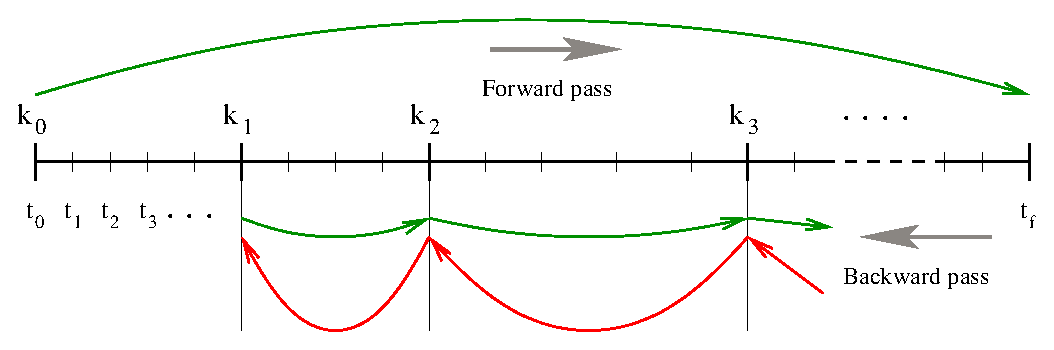
\includegraphics[width=4in]{ckpnt}}
\caption {Illustration of the checkpointing algorithm for generation of 
  the forward solution during the integration of the adjoint system.}
\label{f:ckpnt}
\end{figure}

This approach transfers the uncertainty in the number of integration
steps in the forward integration phase to uncertainty in the final
number of checkpoints.  However, $N_c$ is much smaller than the number
of steps taken during the forward integration, and there is no major
penalty for writing/reading the checkpoint data to/from a temporary
file.
%
Note that, at the end of the first forward integration stage, interpolation
data are available from the last checkpoint to the end of the interval
of integration.  If no checkpoints are necessary ($N_d$ is larger than the 
number of integration steps taken in the solution of (\ref{e:ivp_p})),
the total cost of an adjoint sensitivity computation can be as low as one forward
plus one backward integration.
%
In addition, {\cvodes} provides the capability of reusing a set of checkpoints
for multiple backward integrations, thus allowing for efficient computation of
gradients of several functionals (\ref{e:G}).

\bigskip

\index{adjoint sensitivity analysis!implementation in {\cvodes}|(}
Finally, we note that the adjoint sensitivity module in {\cvodes} provides the
necessary infrastructure to integrate backwards in time any ODE terminal value
problem dependent on the solution of the IVP (\ref{e:ivp_p}), including
adjoint systems (\ref{e:adj_eqns}) or (\ref{e:adj1_eqns}), as well as any other
quadrature ODEs that may be needed in evaluating the integrals in (\ref{e:dGdp}) 
or (\ref{e:dgdp}). In particular, for ODE systems arising from semi-discretization
of time-dependent PDEs, this feature allows for integration of either the 
discretized adjoint PDE system or the adjoint of the discretized PDE.
\index{adjoint sensitivity analysis!implementation in {\cvodes}|)}
\index{adjoint sensitivity analysis!mathematical background|)}

%----------------------------------------
\section{Second-order sensitivity analysis}\label{ss:hess_sensi}
%----------------------------------------
\index{second-order sensitivity analysis}
In some applications (e.g., dynamically-constrained optimization) it may
be desirable to compute second-order derivative information. Considering 
the ODE problem (\ref{e:ivp_p}) and some model output
functional,\footnote{For the sake of simplifity in presentation, we do not 
include explicit dependencies of $g$ on time $t$ or parameters $p$.
Moreover, we only consider the case in which the dependency of the original
ODE (\ref{e:ivp_p}) on the parameters $p$ is through its initial conditions only.
For details on the derivation in the general case, see~\cite{OzBa:05}.}
$g(y)$ then the Hessian $d^2g/dp^2$ can be obtained in a forward sensitivity
analysis setting as
\begin{equation*}
\frac{d^2 g}{d p^2} = \left(g_y \otimes I_{N_p} \right ) y_{pp} + y_p^T g_{yy} y_p \, ,
\end{equation*}
where $\otimes$ is the Kronecker product. The second-order sensitivities are
solution of the matrix ODE system:
\begin{equation*}
  \begin{split}
    & {\dot y}_{pp} = \left( f_y \otimes I_{N_p} \right) \cdot y_{pp} + 
    \left( I_N \otimes y_p^T \right) \cdot f_{yy} y_p \\
    & y_{pp}(t_0) = \frac{\partial^2 y_0}{\partial p^2} \, ,
  \end{split}
\end{equation*}
where $y_p$ is the first-order sensitivity matrix, the solution of $N_p$ 
systems (\ref{e:sens_eqns}), and $y_{pp}$ is a third-order tensor.
%%
It is easy to see that, except for situations in which the number of parameters
$N_p$ is very small, the computational cost of this so-called {\em forward-over-forward} 
approach is exorbitant as it requires the solution of $N_p + N_p^2$ additional
ODE systems of the same dimension $N$ as (\ref{e:ivp_p}).

A much more efficient alternative is to compute Hessian-vector products using
a so-called {\em forward-over-adjoint} approach. This method is based on using
the same ``trick'' as the one used in computing gradients of pointwise
functionals with the adjoint method, namely applying a formal directional forward 
derivation to one of the gradients of (\ref{e:dGdp}) or (\ref{e:dgdp}). With that,
the cost of computing a full Hessian is roughly equivalent to the cost of computing
the gradient with forward sensitivity analysis.  However,
Hessian-vector products can be cheaply computed with one additional adjoint solve.
Consider for example, $G(p) = \int_{t_0}^{t_f} g(t,y) \, dt$.
It can be shown that the product between the Hessian of $G$ (with respect to the 
parameters $p$) and some vector $u$ can be computed as
\begin{equation*}
  \frac{\partial^2 G}{\partial p^2} u = 
  \left[ \left(\lambda^T \otimes I_{N_p} \right) y_{pp}u + y_p^T \mu \right]_{t=t_0} \, ,
\end{equation*}
where $\lambda$, $\mu$, and $s$ are solutions of
\begin{equation}
  \begin{split}
    &-\dot\mu = f_y^T\mu + \left(\lambda^T \otimes I_n \right) f_{yy} s + g_{yy} s\, ; \quad \mu(t_f) = 0 \\
    &-\dot\lambda = f_y^T\lambda + g_y^T \, ; \quad \lambda(t_f) = 0 \\
    &\dot s = f_y s\, ; \quad s(t_0) = y_{0p} u
  \end{split}
\end{equation}
In the above equation, $s = y_p u$ is a linear combination of the columns of the
sensitivity matrix $y_p$.  The {\em forward-over-adjoint} 
approach hinges crucially on the fact that $s$ can be computed at the cost of 
a forward sensitivity analysis with respect to a single parameter (the last 
ODE problem above) which is possible due to the linearity of the forward
sensitivity equations (\ref{e:sens_eqns}).

Therefore, the cost of computing the Hessian-vector product is roughly
that of two forward and two backward integrations of a system of ODEs of size $N$.
For more details, including the corresponding formulas for a pointwise model
functional output, see~\cite{OzBa:05}.

\bigskip

\index{second-order sensitivity analysis!support in {\cvodes}|(}
To allow the {\em foward-over-adjoint} approach described above, {\cvodes}
provides support for:
\begin{itemize}
\item the integration of multiple backward problems depending on the same
  underlying forward problem (\ref{e:ivp_p}), and
\item the integration of backward problems and computation of backward quadratures
  depending on both the states $y$ and forward sensitivities (for this particular 
  application, $s$) of the original problem (\ref{e:ivp_p}).
\end{itemize}
\index{second-order sensitivity analysis!support in {\cvodes}|)}
